\subsection{Brainstorming}\label{subsec:brainstorming}

Before starting on the actual design, the group agreed to have one brainstorming session, where everyone would share
their ideas on how the user interface should look.
Each group member presented their ideas either verbally or through sketches.
From those ideas, the group agreed on a number of key features that the user interface should have.
Everyone agreed that the final interface should be in the form of a dashboard, and that the data from
the~\acrshort{epos} should be visualized in the form of a chart.

\begin{figure}[H]
    \centering
    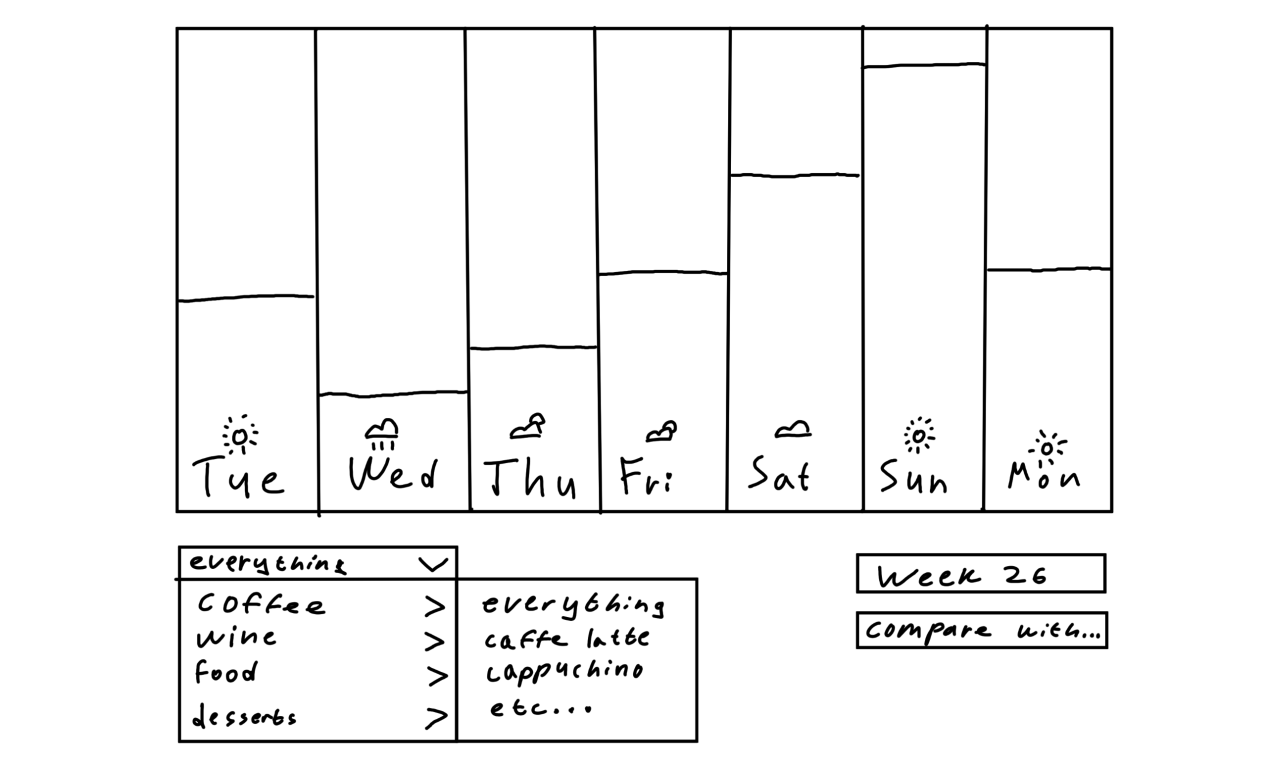
\includegraphics[width=\textwidth]{design-early.png}
    \caption{An example of an early chart.
    }\label{fig:design-early}
\end{figure}

The team decided on prioritizing two charts: A bar chart and a heatmap.
The functionality and choice rationale for these charts are explained in
Section~\ref{subsubsec:relevant-visualization-types}.
Figure~\ref{fig:design-early} shows an early prototype of a bar chart.
The designs and ideas were shared with the client, who approved of the direction the group was taking.
